\subsection{Performance in Trace-Driven Simulations}
\label{sec:performance_large_scale}

%\subsubsection{Benchmarks' performance in simulations}

To verify the correctness of the large-scale simulator, we replayed the BB trace logs from cluster experiments in the simulator.
Table \ref{tbl:speed_up_sim} shows the factors of improvement in completion times of \burstq jobs for BB workload in simulation that are consistent with that from our cluster experiments (Table \ref{tbl:speed_up}). 

\begin{table}[!t]
\small
\centering
\begin{tabular}{|c|c|c|c|c|c|c|} \hline
\multirow{2}{*}{Workload} &  \multicolumn{5}{c}{Number of {\batchq}s} & \\ \hhline{~------}
 & 1 & 2 & 4 & 8 & 16 & 32 \\ \hline \hline
BB & 1.08  & 1.56 & 2.32 & 4.09 & 7.28 & 16.61  \\ \hline 
TPC-DS & 1.06 & 1.38 & 1.66 & 2.93 & 5.16 & 10.40 \\ \hline 
TPC-H  & 1.01 & 1.28 & 1.92 & 3.04 & 5.50 & 11.35 \\ \hline 
\end{tabular}
\caption{[Simulation] Factors of improvement by \name across various workloads w.r.t the number of {\batchq}s.} 
\label{tbl:speed_up_sim}
\end{table}

\name significantly improves over DRF when we have more {\batchq}s.
We note that the factors of improvement for TPC-DS and TPC-H in the simulation are less that of the cluster experiments.
It turns out that DRF in TCP-DS and TPC-H suffers from the allocation overheads that our simulation does not capture.
The allocation overheads for the \burstq jobs in TPC-DS and TPC-H are large because they have more phases than the \burstq jobs in BB (only 2 phases).

%\subsubsection{Admission control for Multiple LQs}
\label{sec:admission_sim}

\begin{figure}[!h]
    \centering
    
\includegraphics[width=0.8\linewidth]{fig/res_usage_b1i3_legend} 
    \vspace{-0.2cm}
    \subfloat[DRF: \burstq-0, \burstq-1, \burstq-2 are unhappy with high latency.]{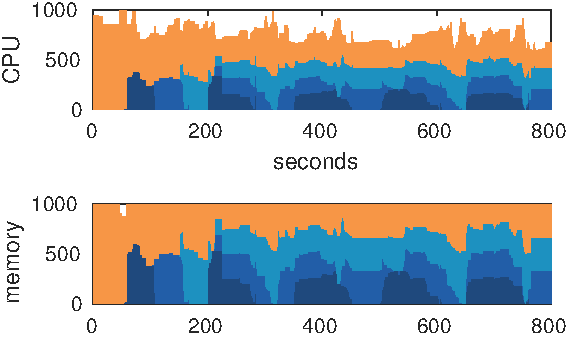
\includegraphics[width=0.8\linewidth]{fig/b1i3_res_usage_drf} \label{fig:admission_drf}} 
    \vspace{-0.1cm}
    \subfloat[SP: \batchq-0 is starving of resources.]{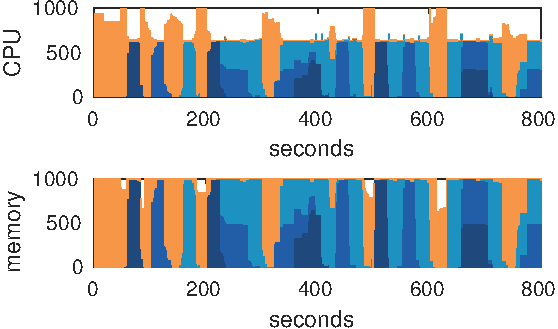
\includegraphics[width=0.8\linewidth]{fig/b1i3_res_usage_strict} \label{fig:admission_strict}}
    \vspace{-0.1cm}            
    \subfloat[N-\name: Only {\burstq}-0 and {\batchq}-0 are happy.]{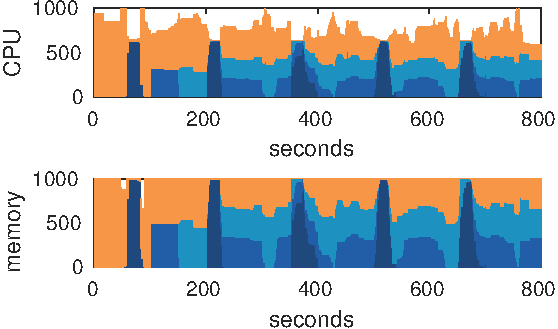
\includegraphics[width=0.8\linewidth]{fig/b1i3_res_usage_Hard} \label{fig:admission_hard}}
    \vspace{-0.1cm}    
    \subfloat[\name: {\burstq}-0, {\burstq}-1 and {\batchq}-1 are happy.]{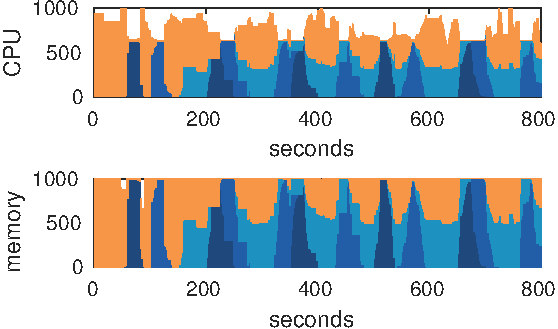
\includegraphics[width=0.8\linewidth]{fig/b1i3_res_usage_speedfair} \label{fig:admission_speedfair}}
    \vspace{-0.1cm}    
    \caption{[Simulation] DRF and SP fail to guarantee both performance and fairness simultaneously. \name gives the best performance to \burstq-0, near optimal performance for \burstq-1, and maintains fairness among 4 queues. \burstq-2 requires too much resource, so its performance cannot be guaranteed.}
    \vspace{-0.5cm}    
    \label{fig:admission_control}
\end{figure}


To demonstrate how \name works with multiple {\burstq}s, we set up 3 {\burstq}s (\burstq-0, \burstq-1, and \burstq-2) and a single \batchq (TQ-0).
The jobs \batchq-0 are queued up at the beginning while \burstq-0, \burstq-1, and \burstq-2 arrive at 50, 100, and 150 seconds, respectively.
The periods of {\burstq}-0, {\burstq}-1, and {\burstq}-2 are 150, \diff{110}, and 60 secs. All the {\burstq}s jobs have the identical demand and task durations.
The TQ jobs are chosen from the BB benchmark.
\name admits {\burstq}-0 to the Hard Guarantee class, {\burstq}-1 to the Soft Guarantee class, and {\burstq}-2 to the Elastic class.

Figure \ref{fig:admission_control} shows the resource usage (CPU and memory) for each queue across four schedulers, i.e., DRF, SP, N-\name and \name.
The capacity of CPU or memory is 1000 nodes.
As an instantaneously fair scheduler, DRF continuously maintains the fair share for all queues as in Figure \ref{fig:admission_drf}.
Since \burstq-2 requires a lot of resources, SP makes \batchq-0 starving for resources (Figure \ref{fig:admission_strict}). N-\name provides \burstq-0 with resource guarantee and it fairly share the resources to \burstq-1, \burstq-2, and \batchq-0 (Figure \ref{fig:admission_hard}).
\name provides hard guarantee to \burstq-0 and soft guarantee to \burstq-1 as in Figure \ref{fig:admission_speedfair}.
The soft guarantee allows \burstq-1 performs better than using N-\name.
Since \burstq-2 demands too much resources, \name treats it like \batchq-0.

Figure \ref{fig:avg_multi_queue} shows the average completion time of jobs on each queue across the four schedulers.
The performance of DRF for \burstq jobs is the worst among the four schedulers but it is the best for only \batchq-0.
The performance of SP is good for \burstq jobs but it is the worst for \batchq jobs.
N-\name provides the best performance for \burstq-0 but not \burstq-1 and \burstq-2.
\name is the best among the four schedulers.
The three of four queues, i.e., \burstq-0, \burstq-1, and \batchq-0, significantly benefit from \name.
\name even outperforms SP for \burstq-0 and \burstq-1 jobs and does not hurt any {\batchq}.

\begin{figure}[!h]
    \centering
    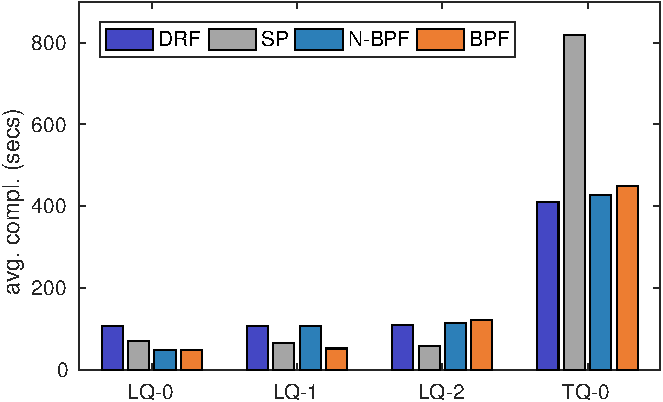
\includegraphics[width=0.8\linewidth]{fig/avg_multi_queuesadmit}
    \caption{[Simulation] \name provides with better performance for {\burstq}s than DRF and N-\name. Unlike SP, \name protects the performance of \batchq jobs.}
    \label{fig:avg_multi_queue}
\end{figure}


%\subsection{Sensitivity Analysis}
%\label{sec:sensitivity_analysis}
%
We use the large-scale simulator to study the impact of estimation errors and non-preemption on \burstq jobs. 
In both cases, \name still outperforms DRF significantly. Results are omitted due to space limit.
%
%\subsubsection{Impact of estimation errors}
%\label{sec:estimation_error_sim}
%
%\name requires users to report their estimated demand for \burstq jobs.
%However, it is challenging to estimate the demand accurately, which naturally results in estimation errors.
%To understand the impact of estimation errors on \name, we assume that estimation errors $e(\%)$ follow the standard normal distribution with zero mean.
%The standard deviation (std.) of estimation errors lines in $[0, 50]$.
%To adopt the estimation errors, we update the task demand and durations of \burstq jobs as $ {task}_{new} = {task}_{original}*(1+e/100)$.
%
%Figure \ref{fig:sen_analysis_est_err} shows the impact of estimation errors on the average completion time of \burstq jobs.
%There are 1 single \burstq and 8 {\batchq}s.
%\burstq jobs arrive every 350 seconds.
%\name is robust when the standard deviation of estimation errors vary 0 to 20.
%The \burstq jobs in BB suffer more from the large estimation errors (std. $>30$) than that of TPC-DS and TPC-H.
%The delays are caused by the underestimated jobs because the excessive demand is not guaranteed by the system.
%Meanwhile, the overestimated jobs do not suffer any delays as the guaranteed resource is more than needed.
%Although estimation errors result in performance degradation, the performance of \burstq jobs is still much better than that of DRF (162 seconds).
%%In the case of large errors, users are suggested reporting larger demands and longer stage-1 durations to improve the performance.\todo{Sentence doesn't parse.}
%
%\begin{figure}[!h]
%\centering
%    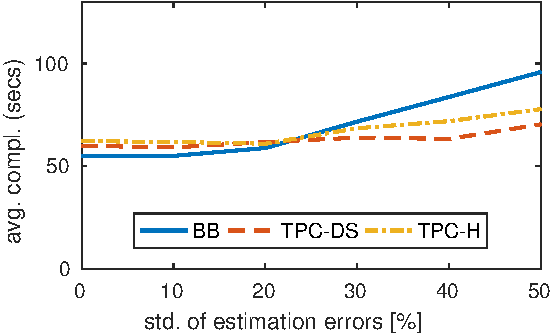
\includegraphics[width=0.7\linewidth]{fig/sen_analysis_est_err}
%\caption{[Simulation] \name's performance degrades with larger estimation errors, yet is still significantly better than DRF (162 secs).}
%\label{fig:sen_analysis_est_err}
%\end{figure}
%
%
%\subsubsection{Impact of non-preemption}
%\label{sec:non_preemption_sim}
%
%To evaluate the impact of non-preemption, we vary the average task durations of {\batchq} jobs.
%The longer task duration is, the longer the task holds its resources.
%In this evaluation, we set up 1 \burstq and 8 {\batchq}s on the simulator.
%Each \burstq job arrives every 350 secs.
%The evaluation is run on three workloads BB, TPC-DS, and TPC-H.
%
%\begin{figure}[!h]
%\centering
%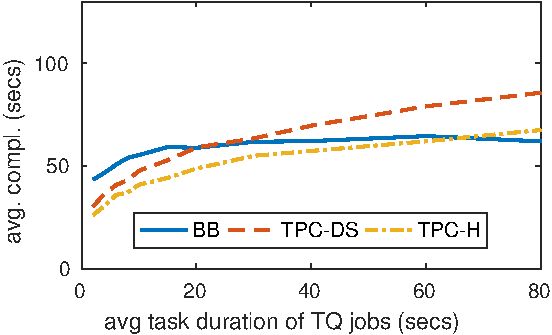
\includegraphics[width=0.7\linewidth]{fig/sen_analysis_task_duration}
%\caption{[Simulation] With longer average task durations, the impact of non-preemption on the performance of \burstq jobs becomes larger. However, the average completion time is still significantly better than that of DRF (162 secs).}
%\label{fig:sen_analysis_task_duration}
%\end{figure}
%
%Figure \ref{fig:sen_analysis_task_duration} shows the impact of average task durations of \batchq jobs on the average completion time of \burstq jobs.
%When we increase the average task durations, the performance of \burstq jobs is degraded.
%Due to the variations of task durations, the BB curve stops increasing from 20, while the TPC-DS and TPC-H curves keep going up.
%Recall the distributions of the task durations in Figure \ref{fig:worklad_cdf}: 70 percent of tasks in BB are very short.
%When the average task durations are more than 20 seconds, there are still a large number of short tasks in BB that allows \name to allocate more resources to \burstq jobs.
%TPC-DS and TPC-H have more variations of task durations that result in increasing delay for \burstq jobs.



